\chapter{Supporting Materials}

\begin{figure}
\centering
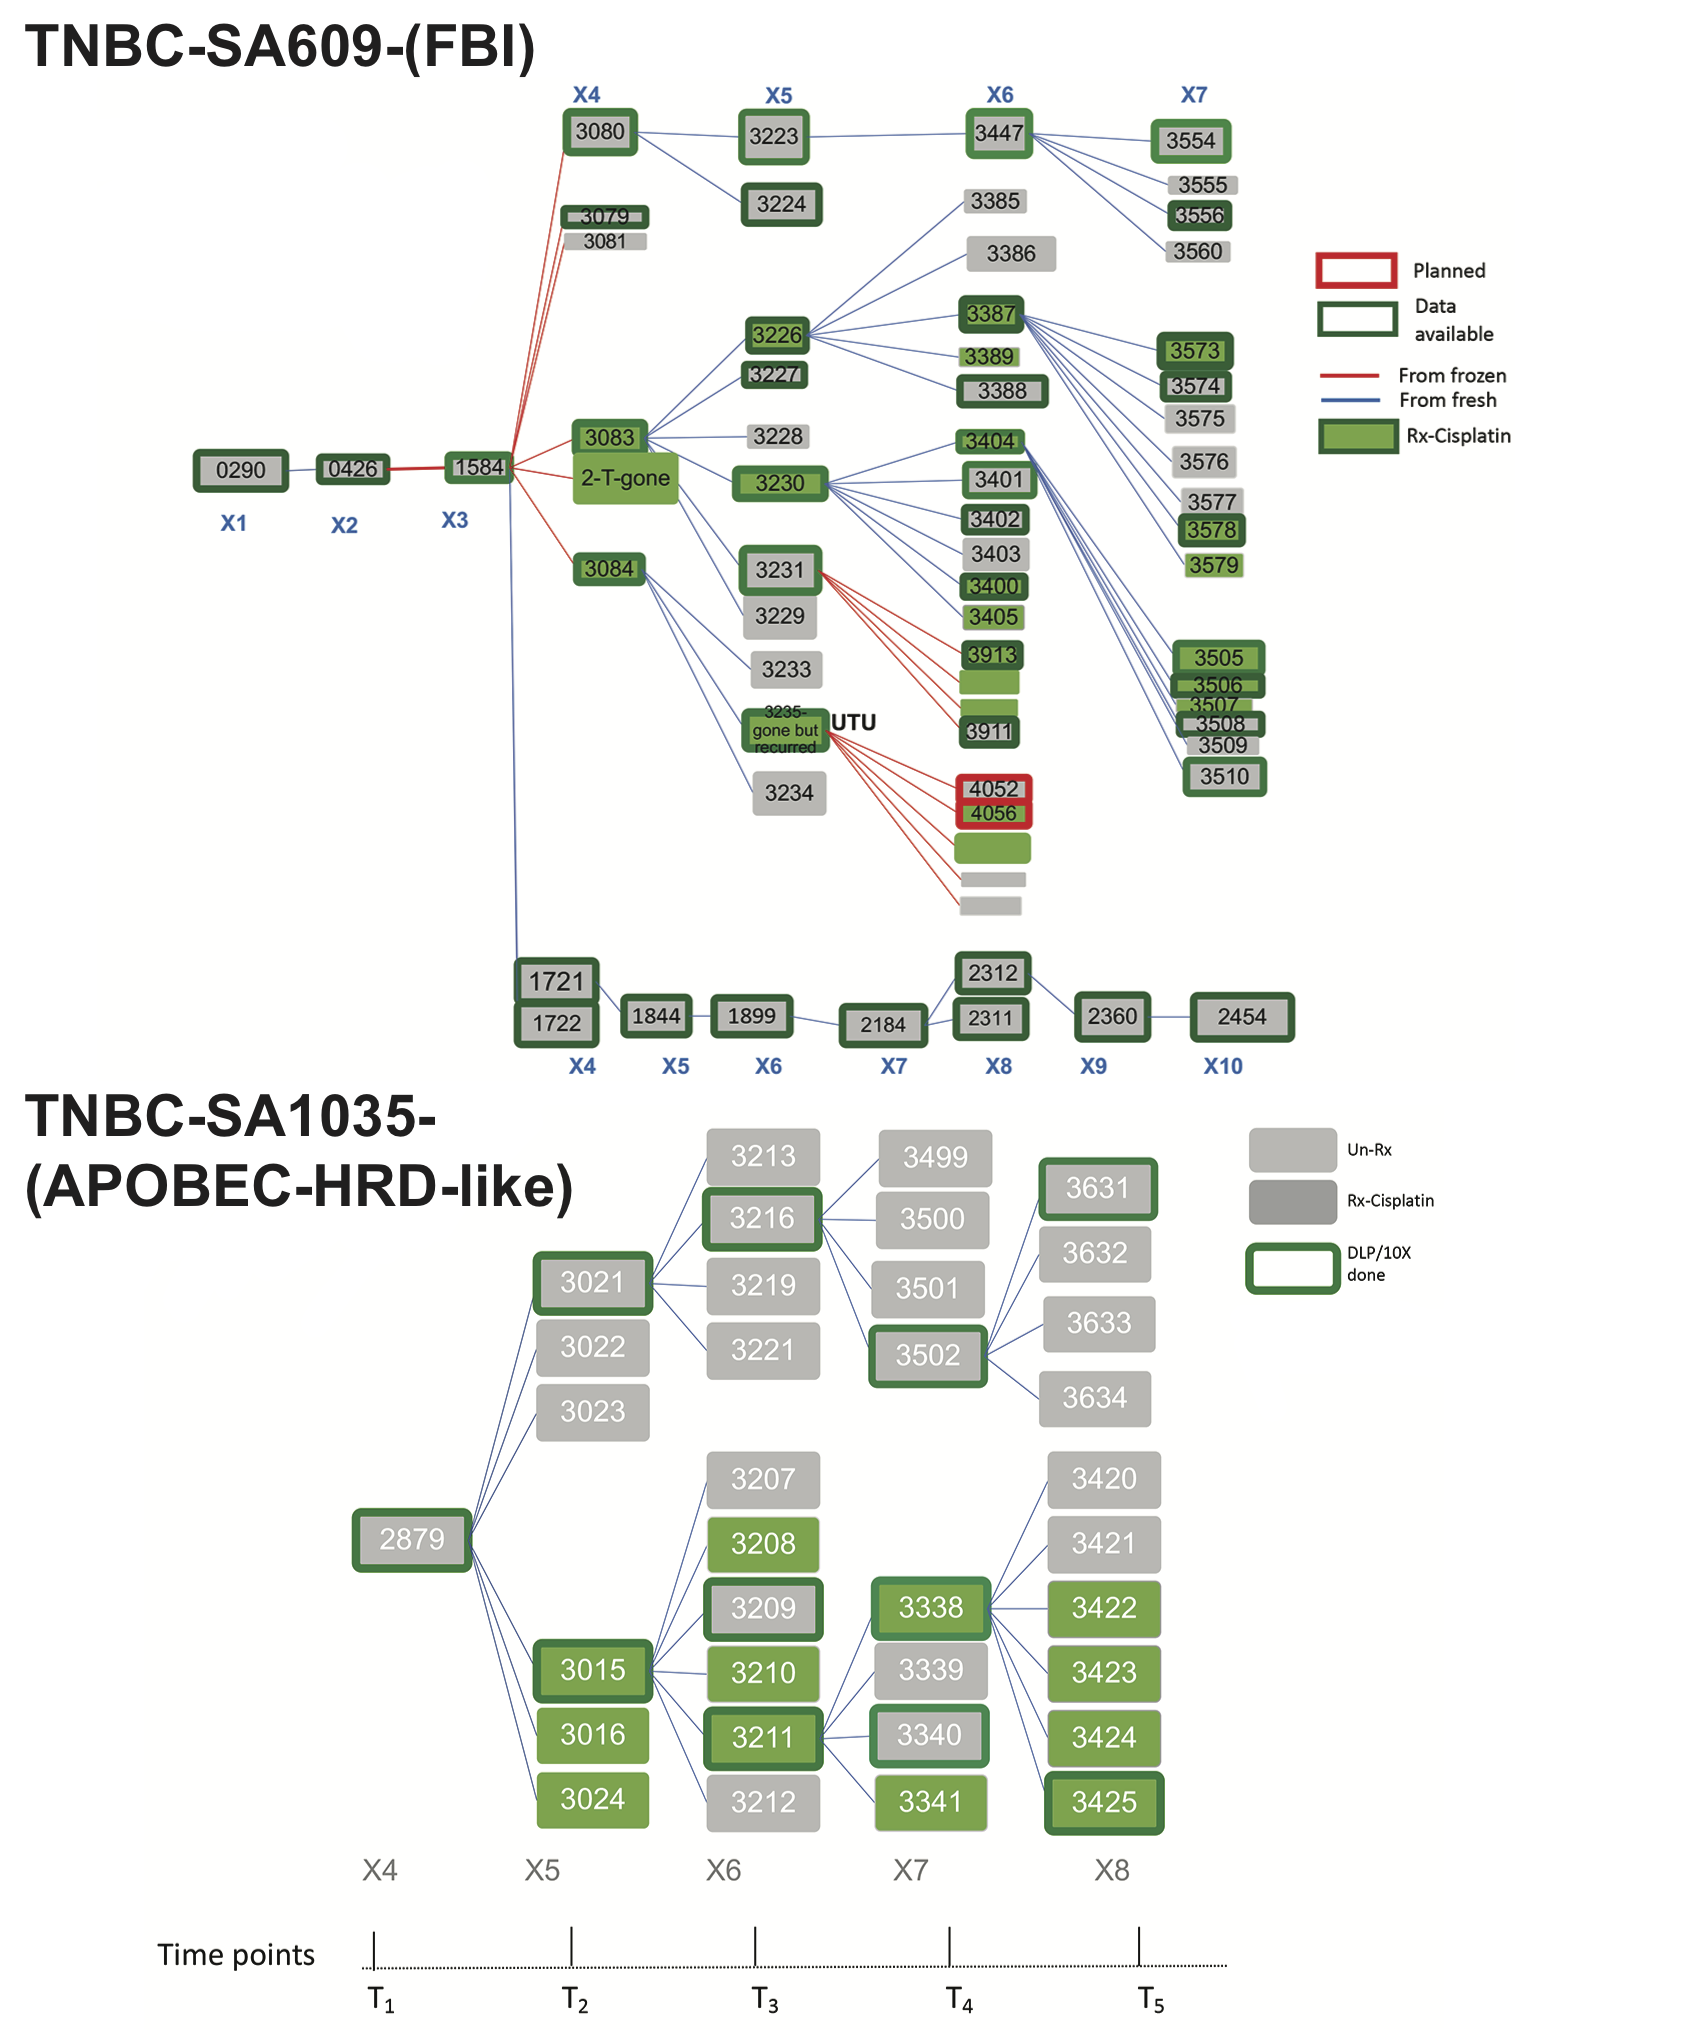
\includegraphics[width=\textwidth]{Figures/SampletreeSA609SA1035.png}
  \caption[Sample ID tree of timeseries TNBC-SA609 and TNBC-SA1035]
	{\small
	\textbf{Sample tree of timeseries TNBC-SA609 and TNBC-SA1035.}

}
    \label{fig:SampletreeSA609SA1035}
    \end{figure}


%-----------------------------------------------------------------
\begin{figure}
\centering
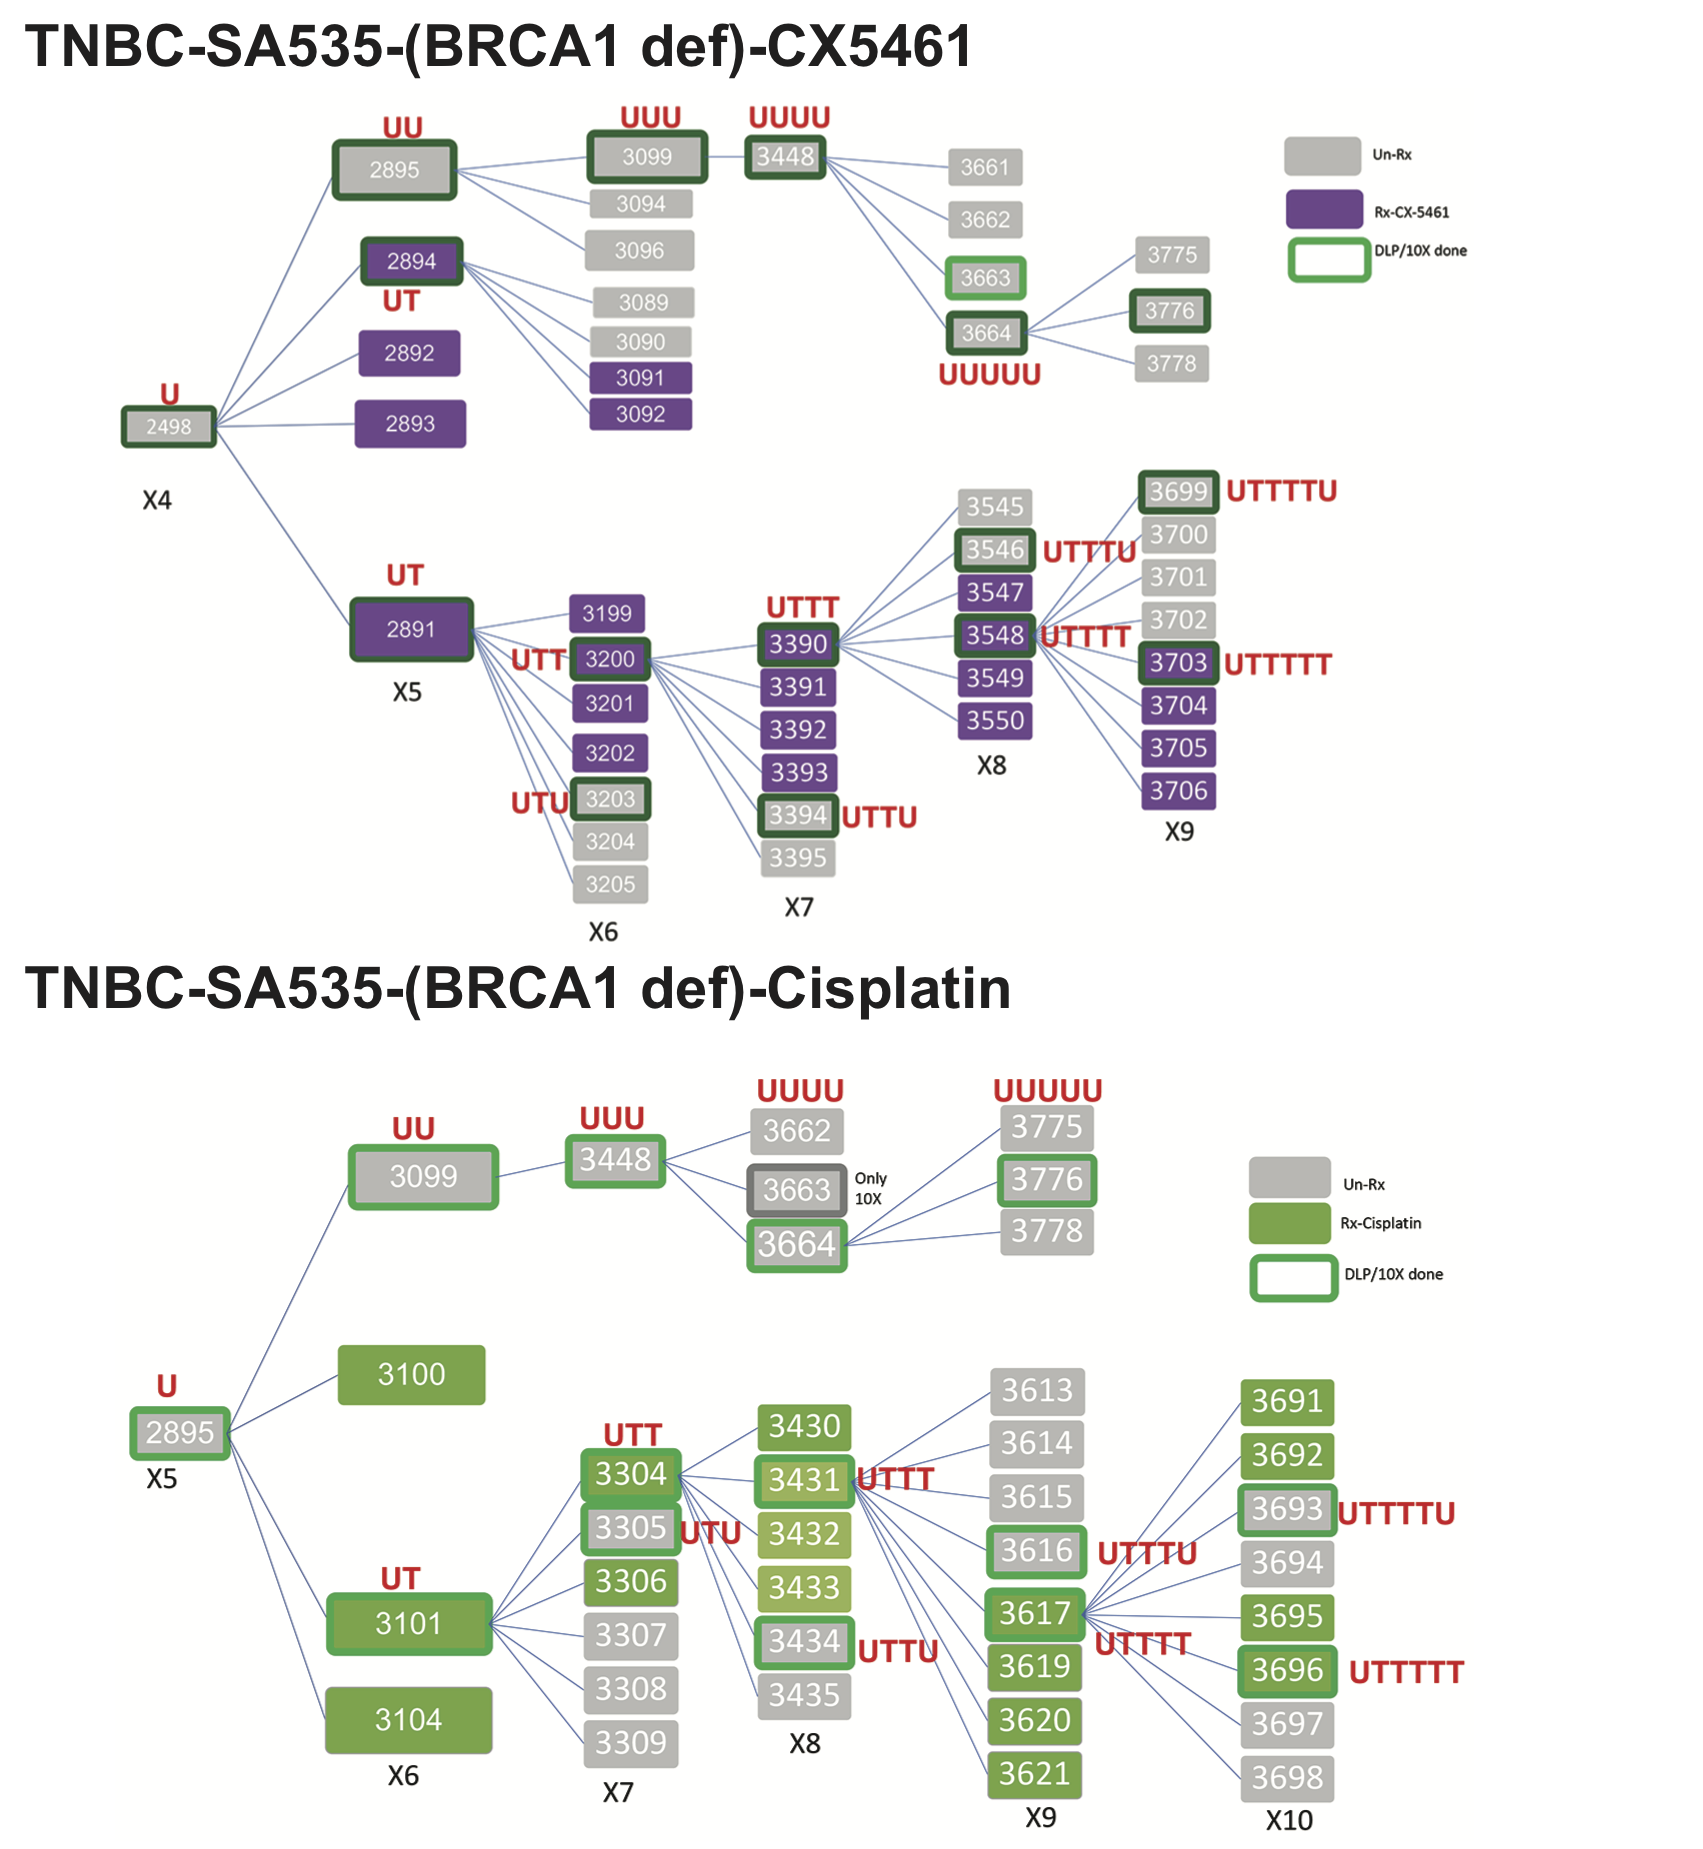
\includegraphics[width=\textwidth]{Figures/SampletreeSA535.png}
  \caption[Sample ID tree of timeseries TNBC-SA609 and TNBC-SA1035]
	{\small
	\textbf{Sample tree of timeseries TNBC-SA535 CX-5461-Rx and Cisplatin-Rx }

}
    \label{fig:SampletreeSA535cisCX}
    \end{figure}







%-----------------------------------------------------------------
\begin{figure}
\centering
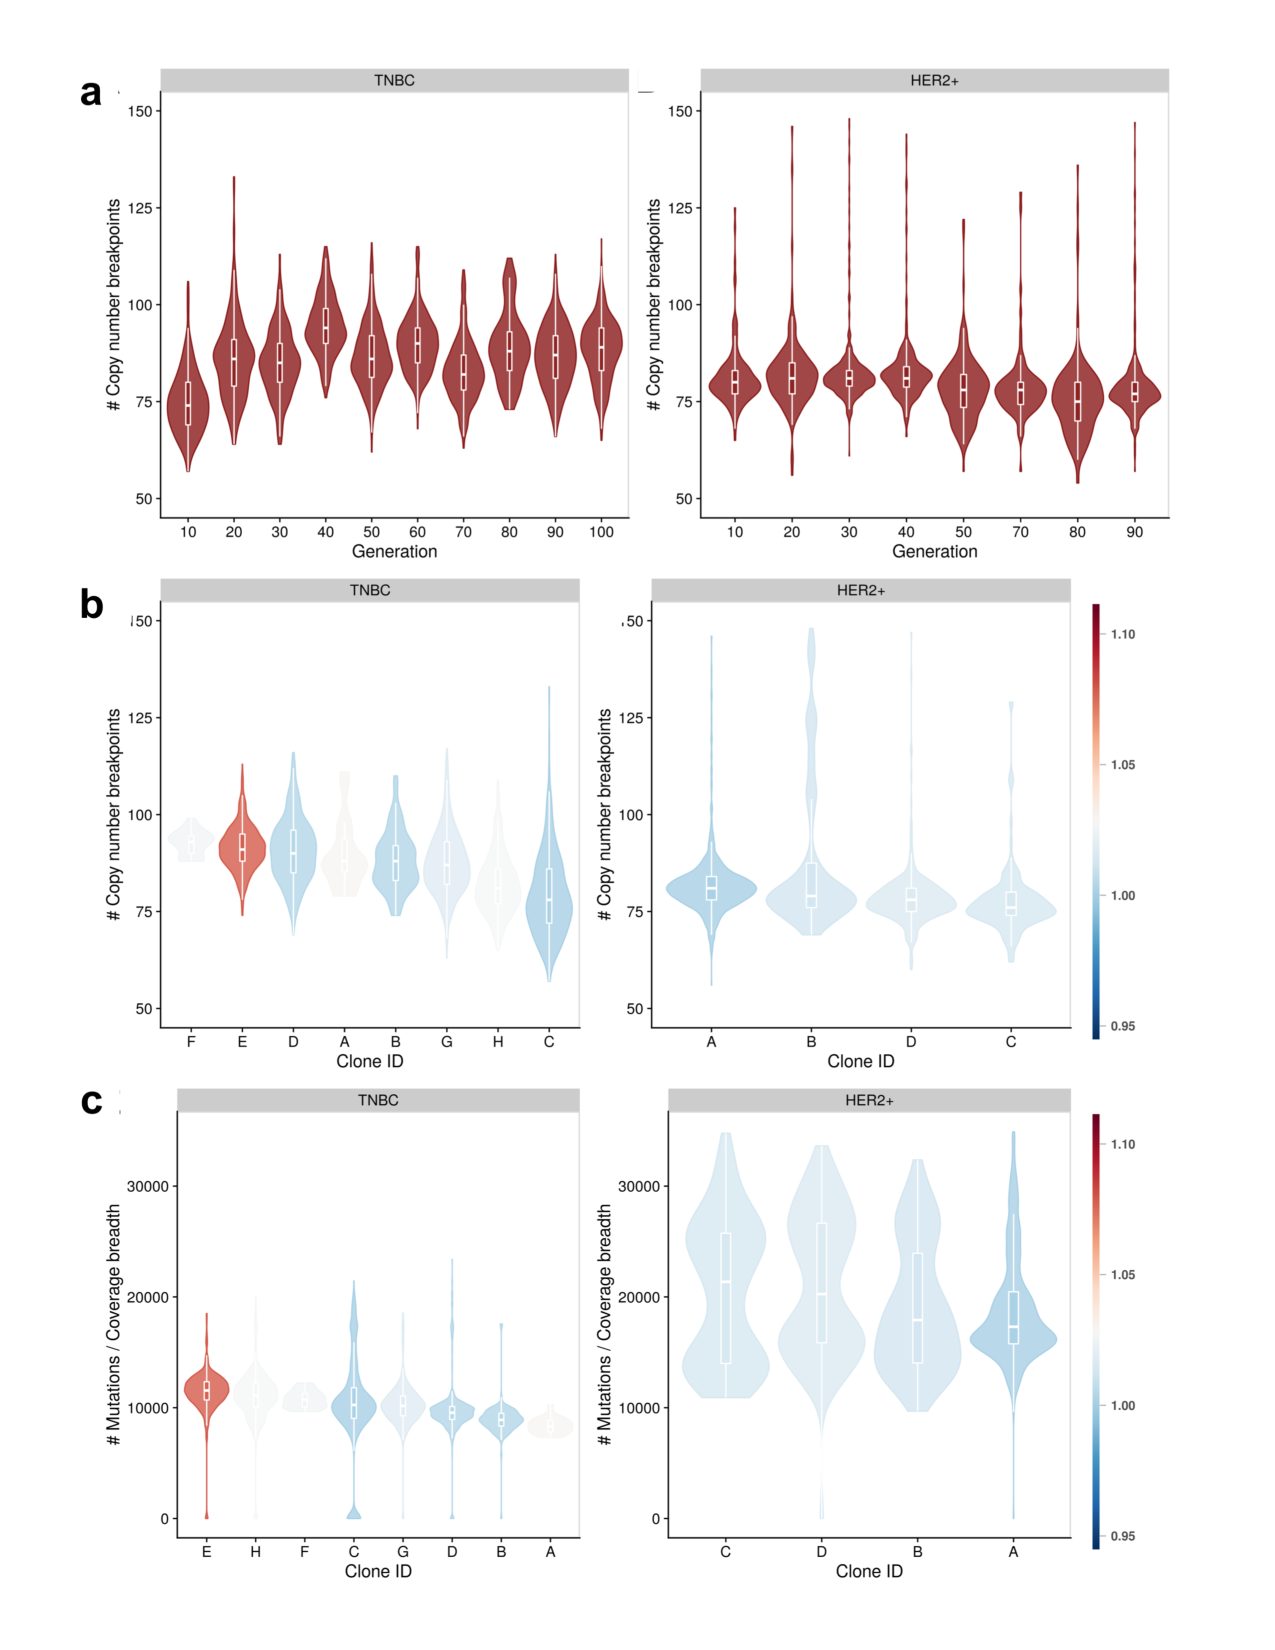
\includegraphics[width=\textwidth]{Figures/chap4/mutationanalysisbreakpoints.pdf}
  \caption[Structural variant and mutation rates of HER2+ and TNBC PDX]
	{\small
	\textbf{Structural variant and mutation rates of HER2+ and TNBC PDX.}
	    \textbf{(a)} Distribution over copy number
breakpoints/cell as a function of generation for left: TNBC, right: HER2+
   \textbf{(b)} Clone specific distributions over copy number breakpoints/cell, coloured by fitness coefficients for left: TNBC, right: HER2+
    \textbf{(c)} Clone specific distributions over point mutations/cell, coloured by fitness coefficients for left:TNBC, right:HER2+
}
    \label{fig:mutationanalysisbreakpoints}
    \end{figure}
%--------------------------------------------------------------------

\begin{figure}
\centering
  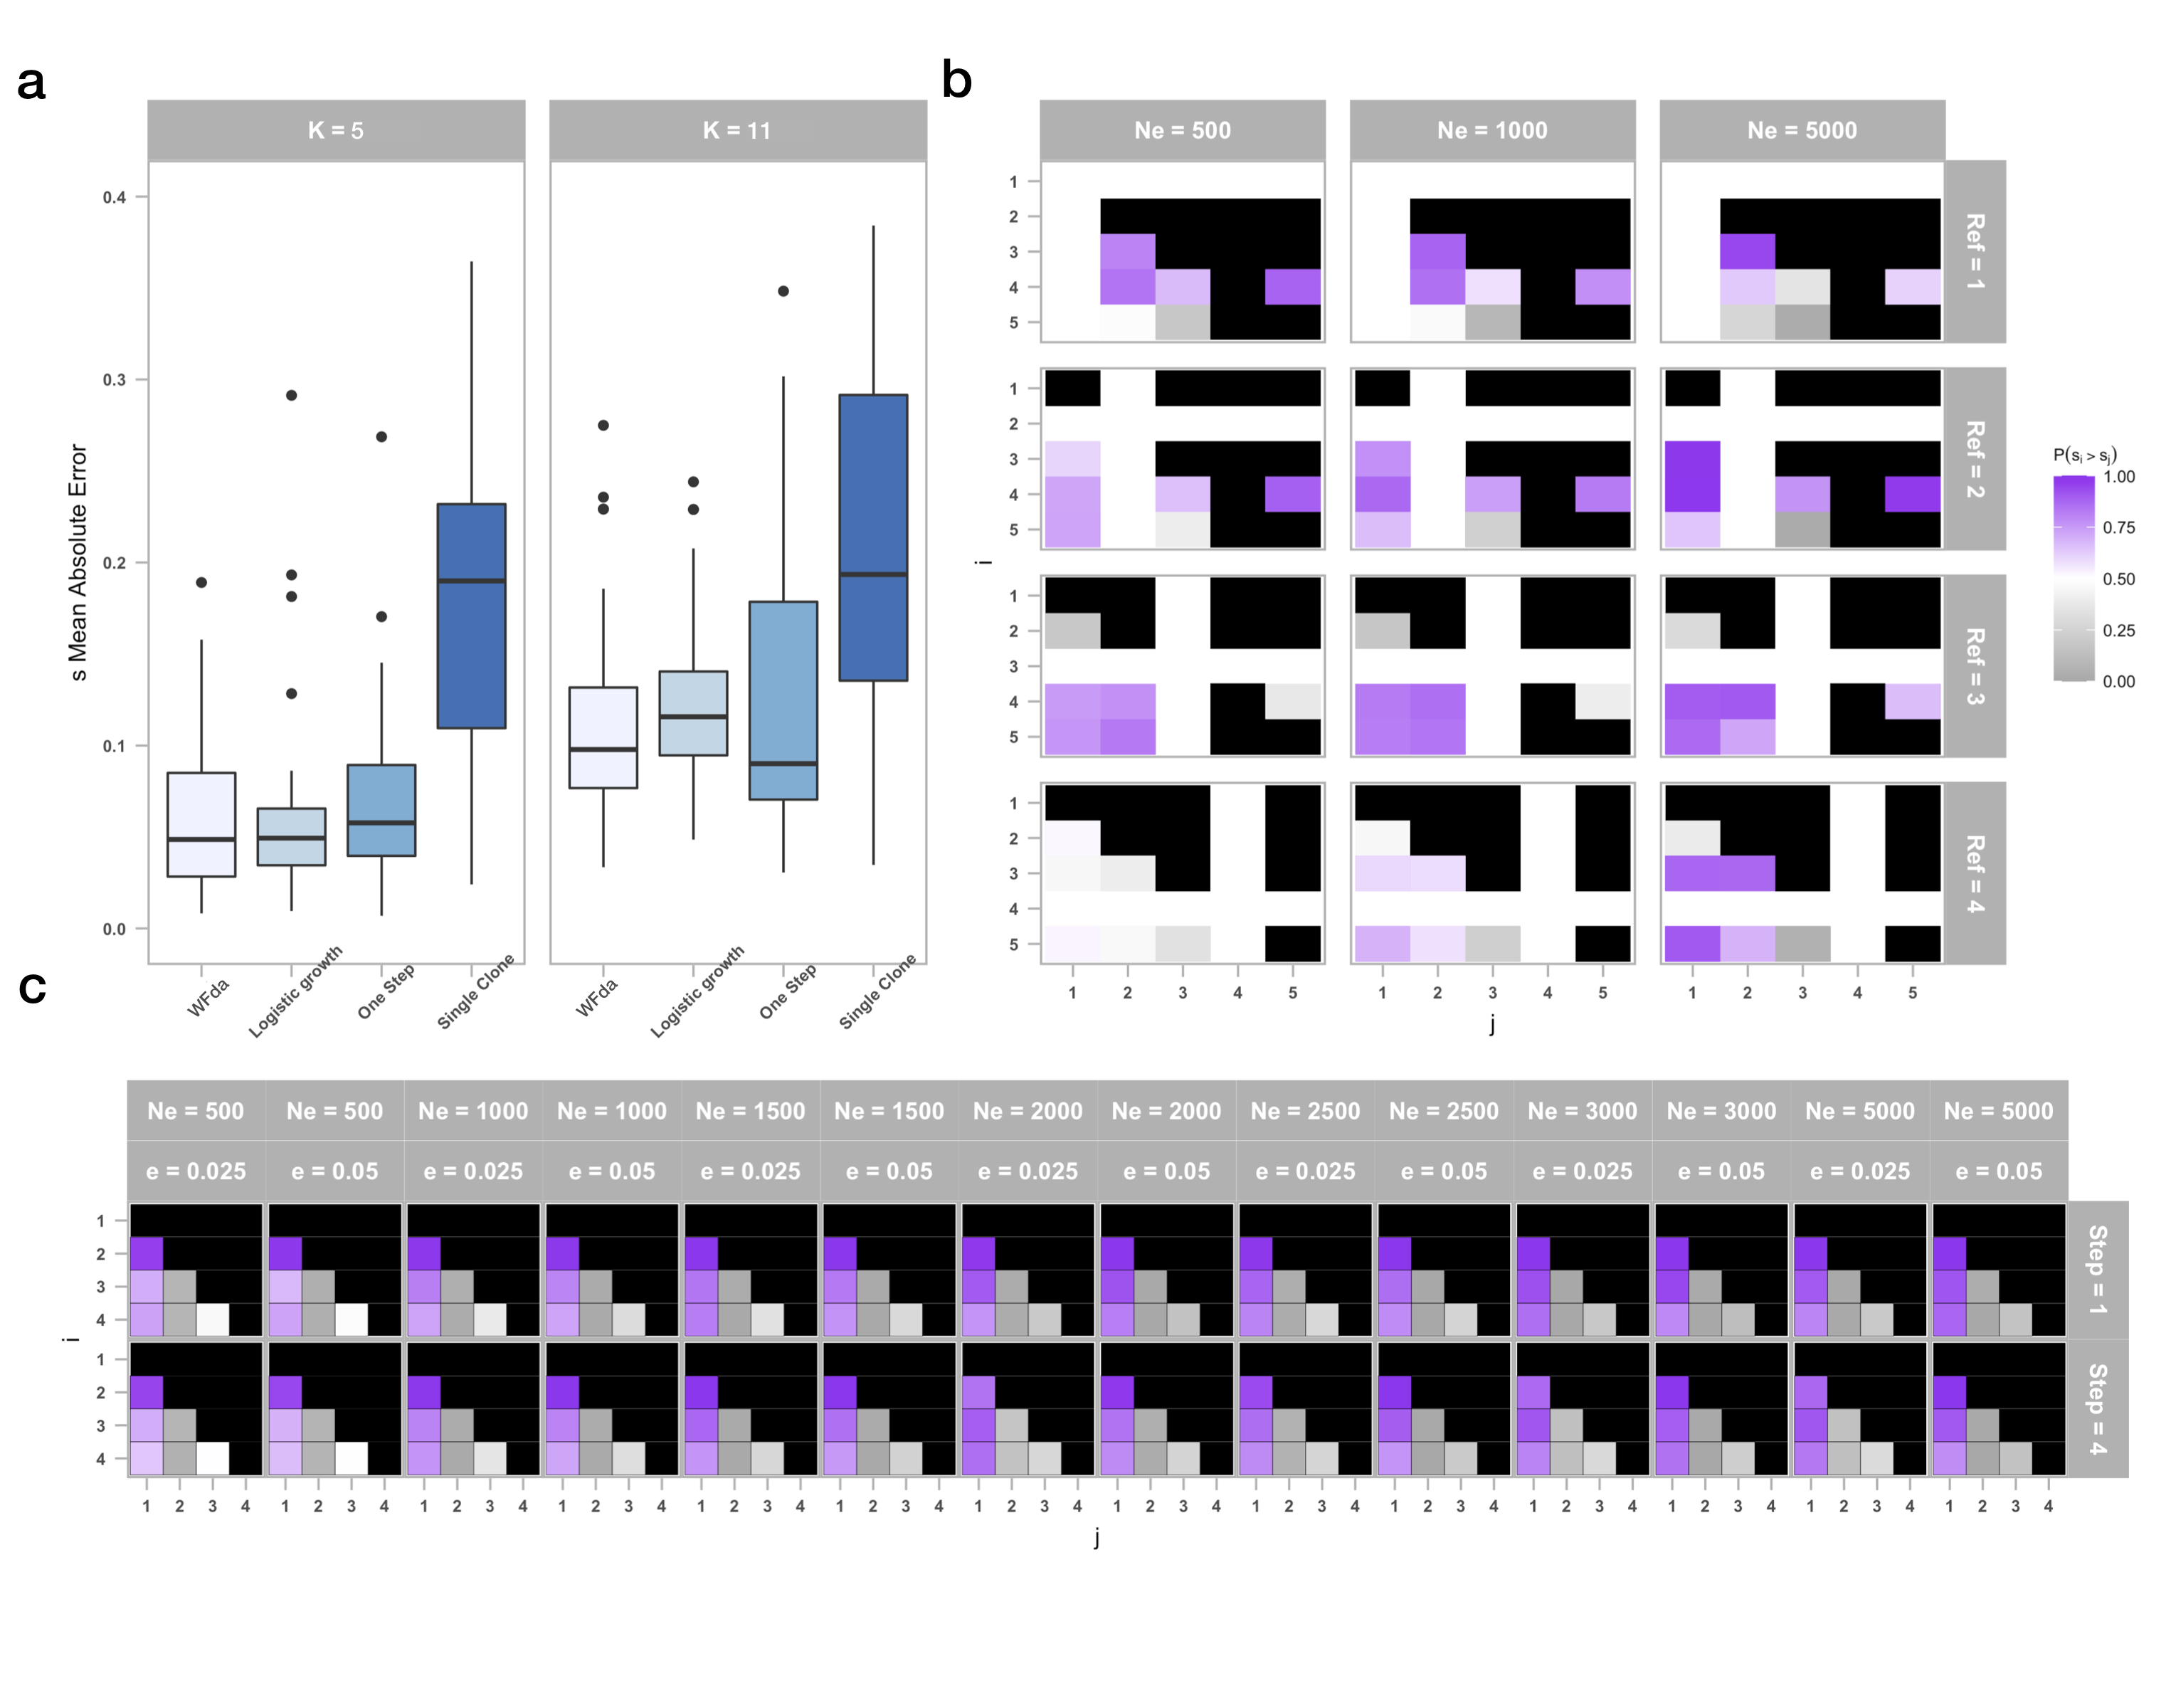
\includegraphics[width=\textwidth]{Figures/simulationspdx.png}
	
\caption[Simulation studies for the \texttt{fitClone} model]
	{\small
	\textbf{Simulation studies for the \texttt{fitClone} model.}
	  (a) Comparison to baseline methods for K = 5 clones (left) and K = 11 clones (right). (b) Posterior ordering of clones based on their inferred posterior selection coefficients across three values of effective population size (columns) and different choice of the reference clone (rows). (c) Posterior ordering of clones across different hyper parameters in the \texttt{fitClone} model. Effective population size in the range of 500 to 5,000 (top column), and observation error (bottom column). Minimum number of interpolations between two observations (rows).}
\label{fig:simulations}
\end{figure}



%---------------------------------------------------------------------------------


%---------------------------------------------------------------
\begin{figure}
\centering
\includegraphics[width=\textwidth]{Figures/chap4/treatedtimeseries.png}
  \caption[TNBC PDX timeseries clonal dynamics under drug perturbations]
	{\small
	\textbf{schematics of complete experimental design of TNBC PDX timeseries for longitudinal single cell evaluation}
	     All nodes representing each PDX tumour were digested to acquire genomes of single cells (~200-600 cells/tumor). Extra replicate tumors at each time point are not shown in the diagram (n=2-4). Grey circles represent un-treated, blue represents Cisplatin treated and grey with blue outline presents drug-holiday samples 
	     \textbf{(a)} SA609-TNBC time series with replicates. DLP+ collected starting from X1 to X10 (Un-Rx line 1). Top grey branch indicating Un-Rx line 2. The middle three branches are cisplatin treated time series replicate branches 
	     \textbf{(b)} SA535-TNBC  showing the tumor nodes taken for DLP+ starting from X5 untreated  \textbf{(c)} SA1035-TNBC  showing the tumor nodes taken for DLP+ starting from X 4 untreated.}
     \label{fig:treatedtimeseriesmanuscript}

\end{figure}

%---------------------------------------------------------------------

 % Table generated by Excel2LaTeX from sheet 'Sheet1'
 \begin{table}[htbp]
   \centering
   \caption{Cisplatin resisatnce related genes from last 10 years literature}
     \begin{tabular}{|l|l|l|l|l|r}
     \hline
     \multicolumn{5}{|l|}{Gene symbols} \\
     \hline
     SETD2 & VDAC & GSH & CLU  & FAS \\
     CREB1 & BAX & GCS & PDK1 & FOS \\
     BRCA1 & BCL & GST & GSR  & GSR \\
     FANCG & BIRC5  & MT & MSH2  & GJA1 \\
     FANCA & CPN & ERCC1 & NOX4  & HSPB1 \\
     POLD1 & CASP & MLH1 & NQO1 & MSH2 \\
     KDM1A & MAPKs & MSH2 & TUBA1A  & NOX4 \\
     BLM & p63 & POLH & VCAM1  & NQO1 \\
     PIK3CA & TP53 & REV3 & VIM  & PTK2 \\
     ERBB2 & XAF1 & REV7 & SLC31A1 & TUBA1A \\
     ERBB3 & DYRK1B & BRCA1 & GST & VCAM1 \\
     CDK4 & ERBB2  & BRCA2 & HMGB & ABCC2  \\
     AKT1 & HSPs & ERK gene & CTR1 & AKT1  \\
     ESR1 & TMEM205 & PI3K & ATP7A & BCL2L1  \\
     TYMS & PDGFR $\beta$ & GREB1 & ATP7B & CASP8  \\
     PIK3CB & IGF1R & ROR2 & MRP2 & BCL2L1 \\
     PTEN & TRP14 & Wnt5a & ADM & CAV1 \\
     IGF1 & RAB7 & STAT3 & AKT1 & ERK gene \\
     NFKB1, 2 & RAB8 & ATF3 & BCL2 & ABCC2 \\
     \hline
     \end{tabular}%
   \label{tab:Cisplatinrelatedgenes}%
 \end{table}%


%-------------------------------------------------------------------
\begin{figure}
\centering
  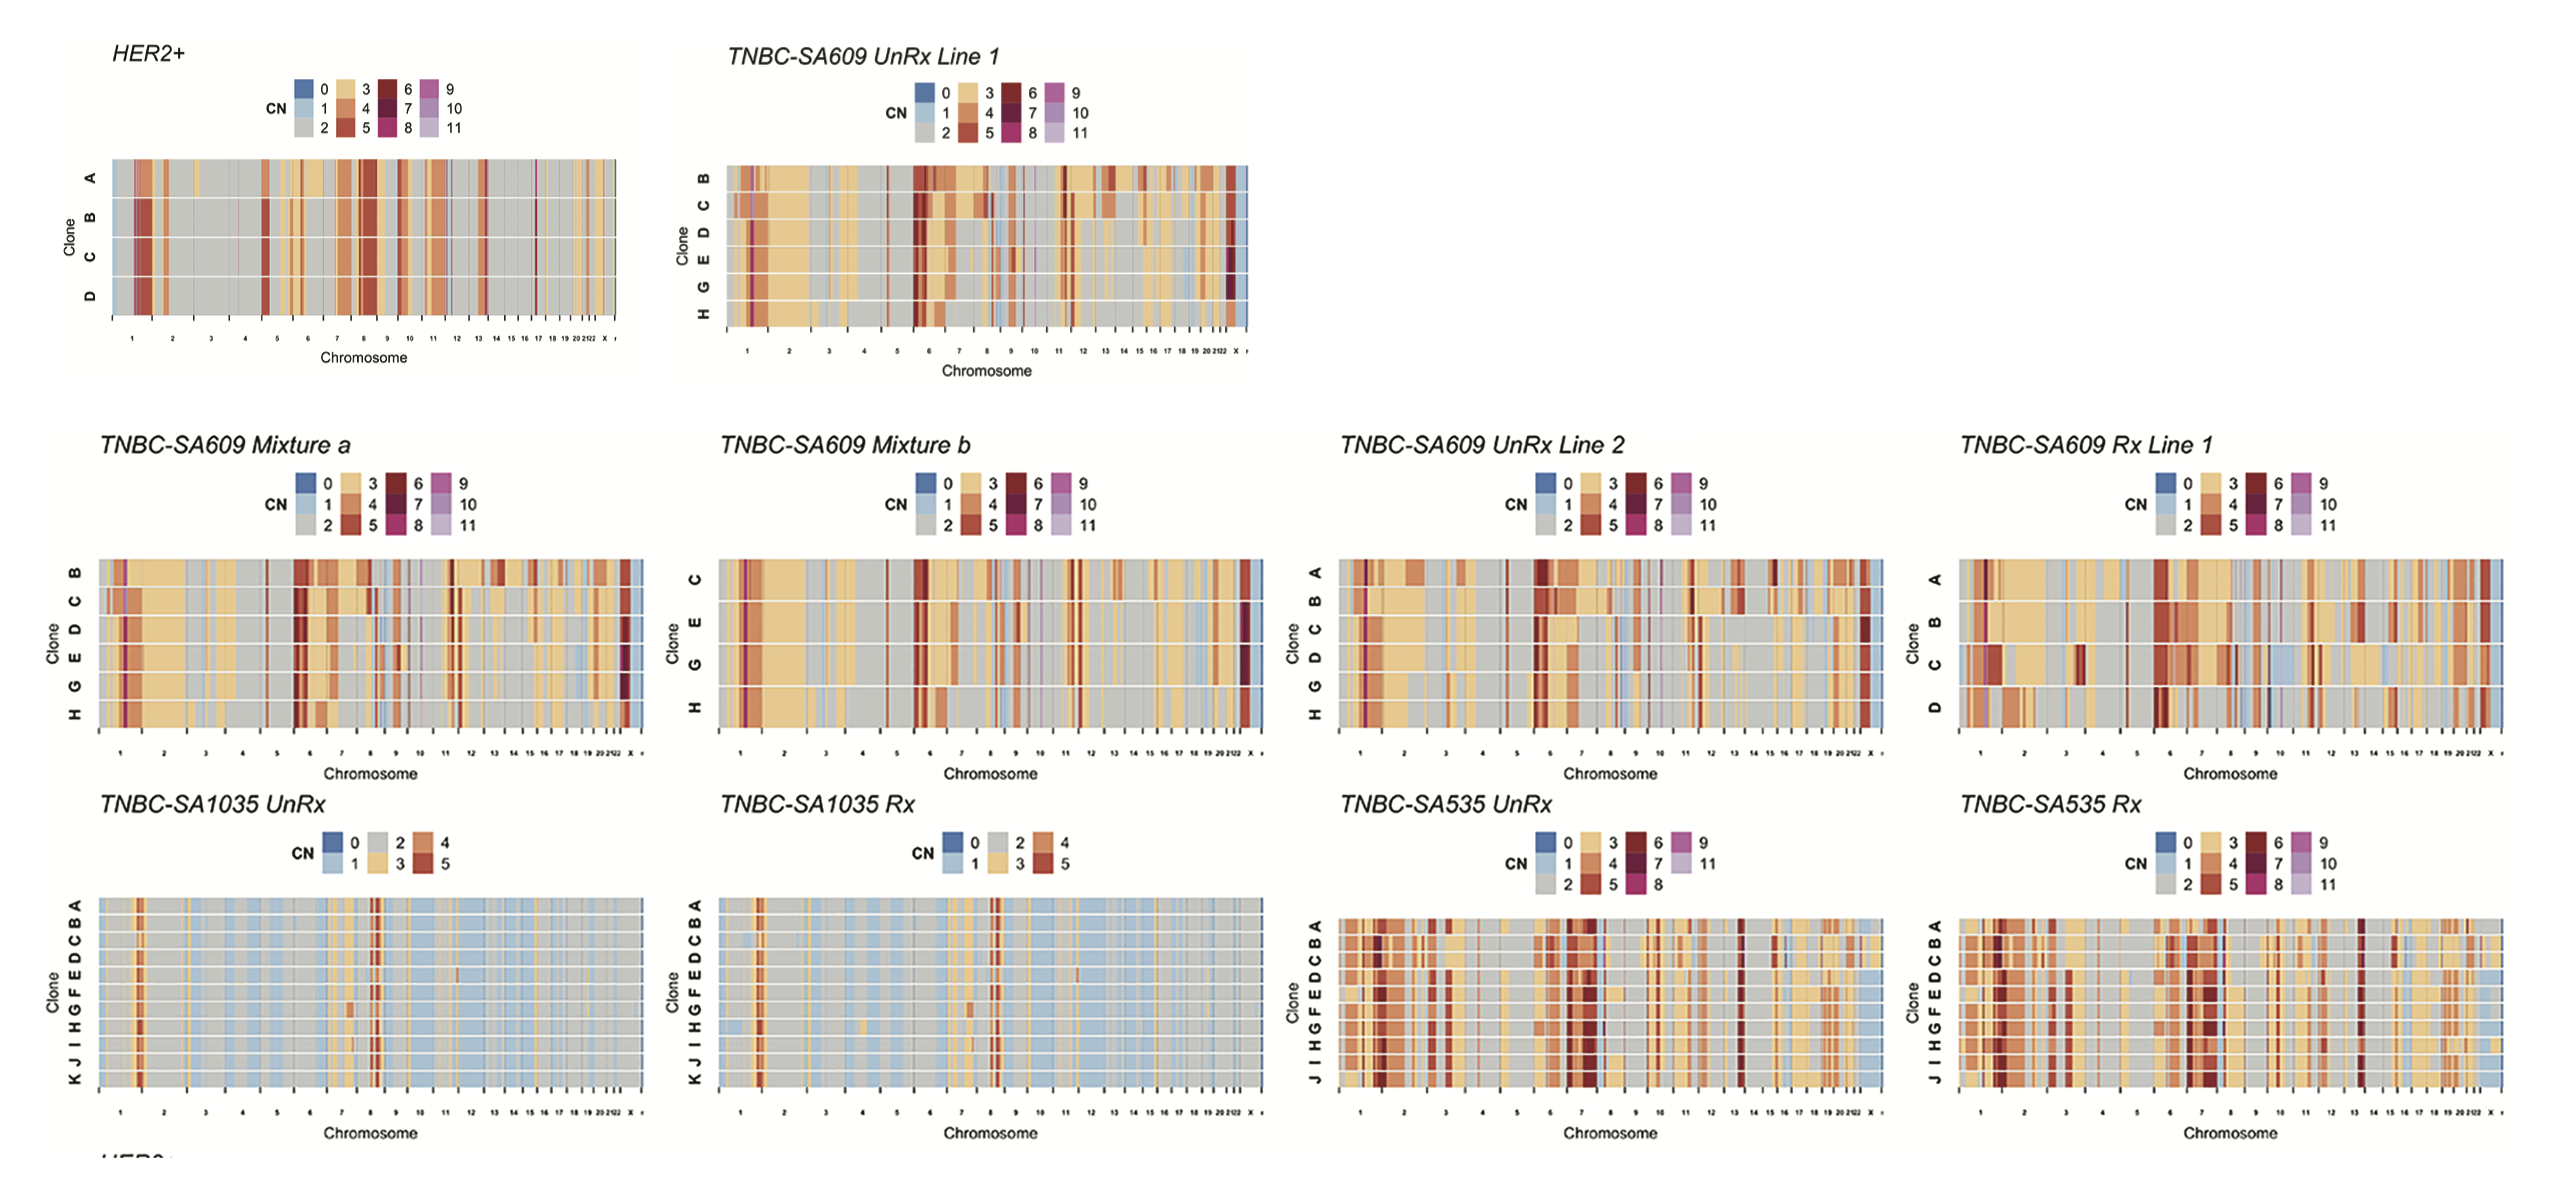
\includegraphics[width=\textwidth]{Figures/chap4/mediangenotypespdx.png}
\caption[Heatmaps of median genotypes]
	{\small
	\textbf{Heatmap representation of per clone median genotypes for TNBC PDX series SA609 UnRx Line 1 (U1), TNBC-SA609 mixtures a and b (Ma and Mb), SA609 UnRx Line 2 (U2), SA609 Rx line 1 (R1), SA1035 and SA535 treated and untreated (Un and Rx)}}.
	  
	 	\label{fig:mediangenotypes}
\end{figure} 
%---------------------------------------------------------------

% Please add the following required packages to your document preamble:
% \usepackage{graphicx}
% \usepackage{lscape}
\begin{landscape}
\begin{table}[]
\caption{TNBC PDX-TMA scoring of IHC staining intensity}
\label{tab:TNBCTMAscoringIHC}
\resizebox{1.5\textwidth}{!}{%
\begin{tabular}{lllllllllllllllllllllll}
Timeseries & Timepoints & Treatment status & Block ID & ER  & ER \% & PR  & PR \% & HER 2  & HER 2 \% & Ki67  & Ki67 \% & EGFR  & EGFR \% & SMA  & SMA \% & CK8  & CK8 \% & CK14 & CK14 \% & CK5/6  & CK5/6 \% & E-cad \\
TNBC-SA609 & X4 & Un-Rx & 3080 & 0 & 0 & 0 & 0 & 0 & 0 & 3+ & 45 & 1+ & 50 & 0 & 0 & 0 & 0 & 0 & 0 & 0 & 0 & 0 \\
TNBC-SA609 & X5 & Un-Rx & 3223 & 0 & 0 & 0 & 0 & 0 & 0 & 3+ & 50 & 1+ & 40 & 0 & 0 & 0 & 0 & 0 & 0 & 0 & 0 & 0 \\
TNBC-SA609 & X6 & Un-Rx & 3447 & 0 & 0 & 0 & 0 & 0 & 0 & 3+ & 45 & 2+ & 30 & 3+ & 0-1 & 0 & 0 & 0 & 0 & 0 & 0 & 0 \\
TNBC-SA609 & X4 & Rx & 3083 & 0 & 0 & 0 & 0 & 0 & 0 & 3+ & 60 & 1+ & 60 & 0 & 0 & 0 & 0 & 0 & 0 & 0 & 0 & 0 \\
TNBC-SA609 & X4 & Rx & 3084 & 0 & 0 & 0 & 0 & 0 & 0 & 3+ & 70 & 1+ & 70 & 0 & 0 & 0 & 0 & 0 & 0 & 0 & 0 & 0 \\
TNBC-SA609 & X5 & Rx & 3230 & 0 & 0 & 0 & 0 & 0 & 0 & 3+ & 45 & 1+ & 50 & 0 & 0 & 0 & 0 & 0 & 0 & 0 & 0 & 0 \\
TNBC-SA609 & X5 & dh & 3231 & 0 & 0 & 0 & 0 & 0 & 0 & 3+ & 35 & 1+ & 75 & 0 & 0 & 0 & 0 & 0 & 0 & 0 & 0 & 0 \\
TNBC-SA609 & X5 & Rx-recur & 3235 & 0 & 0 & 0 & 0 & 0 & 0 & 3+ & 35 & 2+ & 50 & 0 & 0 & 0 & 0 & 0 & 0 & 0 & 0 & 0 \\
TNBC-SA609 & X6 & Rx & 3400 & 0 & 0 & 0 & 0 & 0 & 0 & 3+ & 35 & 1+ & 40 & 0 & 0 & 0 & 0 & 0 & 0 & 0 & 0 & 0 \\
TNBC-SA609 & X6 & dh & 3401 & 0 & 0 & 0 & 0 & 0 & 0 & 3+ & 30 & 1+ & 10 & 0 & 0 & 0 & 0 & 0 & 0 & 0 & 0 & 0 \\
TNBC-SA609 & X6 & Rx & 3404 & 0 & 0 & 0 & 0 & 0 & 0 & 3+ & 35 & 1+ & 40 & 0 & 0 & 0 & 0 & 0 & 0 & 0 & 0 & 0 \\
TNBC-SA609 & X7 & Rx & 3505 & 0 & 0 & 0 & 0 & 0 & 0 & 3+ & 50 & 1+ & 40 & 0 & 0 & 0 & 0 & 0 & 0 & 0 & 0 & 0 \\
TNBC-SA609 & X7 & Rx & 3506 & 0 & 0 & 1+ & 0-1 & 0 & 0 & 3+ & 60 & 1+ & 60 & 0 & 0 & 0 & 0 & 0 & 0 & 0 & 0 & 0 \\
TNBC-SA609 & X7 & dh & 3510 & 0 & 0 & 1+ & 0-1 & 0 & 0 & 3+ & 45 & 1+ & 40 & 0 & 0 & 0 & 0 & 0 & 0 & 0 & 0 & 0 \\
TNBC-SA609 & X5 & Rx & 3226 & 0 & 0 & 0 & 0 & 0 & 0 & 3+ & 45 & 1+ & 35 & 0 & 0 & 0 & 0 & 0 & 0 & 0 & 0 & 0 \\
TNBC-SA609 & X6 & Rx & 3387 & 0 & 0 & 0 & 0 & 0 & 0 & 3+ & 50 & 1+ & 50 & 0 & 0 & 0 & 0 & 0 & 0 & 0 & 0 & 0 \\
TNBC-SA609 & X7 & Rx & 3573 & 0 & 0 & 0 & 0 & 0 & 0 & 3+ & 90 & 3+ & 5 & 0 & 0 & 0 & 0 & 0 & 0 & 0 & 0 & 0 \\
TNBC-SA609 & X7 & Rx & 3578 & 0 & 0 & 0 & 0 & 0 & 0 & 3+ & 90 & 1+ & 10 & 0 & 0 & 0 & 0 & 0 & 0 & 0 & 0 & 0 \\
TNBC-SA609 & X7 & dh & 3508 & 0 & 0 & 0 & 0 & 0 & 0 & 3+ & 35 & 1+ & 35 & 0 & 0 & 0 & 0 & 0 & 0 & 0 & 0 & 0 \\
TNBC-SA609 & X7 & dh & 3577 & 0 & 0 & 0 & 0 & 0 & 0 & 3+ & 80 & 1+ & 0-5 & 0 & 0 & 0 & 0 & 0 & 0 & 0 & 0 & 0 \\
 &  &  &  &  &  &  &  &  &  &  &  &  &  &  &  &  &  &  &  &  &  &  \\
TNBC-SA1035 & X4 & Un-Rx & 2879 & 1+ & 0-1 & 0 & 0 & 0 & 0 & 3+ & 65 & 3+ & 100 & 0 & 0 & 1+ & 25 & 3+ & 10 & 2+ & 10 & 3+ \\
TNBC-SA1035 & X5 & Un-Rx & 3021 & 1+ & 0-1 & 0 & 0 & 0 & 0 & 3+ & 50 & 3+ & 100 & 0 & 0 & 1+ & 5 & 3+ &  & 2+ & 10 & 3+ \\
TNBC-SA1035 & X6 & Un-Rx & 3216 & 1+ & 0-1 & 0 & 0 & 0 & 0 & 2+ & 65 & 3+ & 100 & 0 & 0 & 2+ & 5 & 3+ & 0-1 & 2+ & 0-1 & 3+ \\
TNBC-SA1035 & X7 & Un-Rx & 3502 & 1+ & 0-1 & 0 & 0 & 0 & 0 & 3+ & 70 & 3+ & 100 & 0 & 0 & 1+ & 5 & 3+ & 5 & 2+ & 10 & 3+ \\
TNBC-SA1035 & X8 & Un-Rx & 3631 & 1+ & 0-1 & 0 & 0 & 0 & 0 & 3+ & 80 & 3+ & 100 & 0 & 0 & 1+ & 0-1 & 3+ & 0-1 & 2+ & 1 & 3+ \\
TNBC-SA1035 & X5 & Rx & 3015 & 1+ & 0-1 & 0 & 0 & 0 & 0 & 3+ & 50 & 3+ & 95 & 0 & 0 & 2+ & 70 & 3+ & 10 & 3+ & 40 & 3+ \\
TNBC-SA1035 & X6 & dh & 3209 & 1+ & 0-1 & 0 & 0 & 0 & 0 & 3+ & 60 & 3+ & 100 & 0 & 0 & 2+ & 5 & 3+ & 1 & 2+ & 10 & 3+ \\
TNBC-SA1035 & X6 & Rx & 3211 & 1+ & 0-1 & 0 & 0 & 0 & 0 & 3+ & 50 & 3+ & 100 & 0 & 0 & 2+ & 20 & 3+ & 1 & 2+ & 30 & 3+ \\
TNBC-SA1035 & X7 & Rx & 3338 & 1+ & 0-1 & 0 & 0 & 0 & 0 & 3+ & 80 & 3+ & 100 & 0 & 0 & 1+ & 5 & 3+ & 5-10 & 2+ & 15 & 3+ \\
TNBC-SA1035 & X7 & dh & 3340 & 1+ & 0-1 & 0 & 0 & 0 & 0 & 3+ & 60 & 3+ & 100 & 0 & 0 & 2+ & 5 & 3+ & 1 & 2+ & 10 & 3+ \\
TNBC-SA1035 & X8 & Rx & 3425 & 1+ & 0-1 & 0 & 0 & 0 & 0 & 3+ & 70 & 3+ & 100 & 0 & 0 & 1+ & 5 & 3+ & 1 & 2+ & 5 & 3+ \\
 &  &  &  &  &  &  &  &  &  &  &  &  &  &  &  &  &  &  &  &  &  &  \\
TNBC-SA535 & X6 & Un-Rx & 3099 & 0 & 0 & 0 & 0 & 0 & 0 & 3+ & 25 & 3+ & 90 & 0 & 0 & 2+ & 65 & 0 & 0 & 2+ & 5-10 & 3+ \\
TNBC-SA535 & X7 & Un-Rx & 3448 & 0 & 0 & 0 & 0 & 0 & 0 & 3+ & 30 & 3+ & 100 & 0 & 0 & 2+ & 15 & 0 & 0 & 2+ & 0-1 & 3+ \\
TNBC-SA535 & X6 & Rx & 3101 & 1+ & 0-1 & 0 & 0 & 0 & 0 & 3+ & 35 & 2+ & 95 & 0 & 0 & 2+ & 80 & 3+ & 1 & 2+ & 5 & 3+ \\
TNBC-SA535 & X7 & Rx-cis & 3304 & 0 & 0 & 0 & 0 & 0 & 0 & 3+ & 35 & 2+ & 80 & 0 & 0 & 2+ & 95 & 3+ & 0-1 & 2+ & 1 & 3+ \\
TNBC-SA535 & X7 & dh-cis & 3305 & 0 & 0 & 0 & 0 & 0 & 0 & 3+ & 35 & 2+ & 90 & 0 & 0 & 3+ & 95 & 3+ & 1 & 2+ & 5 & 3+ \\
TNBC-SA535 & X8 & Rx-cis & 3431 & 1+ & 0-1 & 0 & 0 & 0 & 0 & 3+ & 45 & 2+ & 95 & 0 & 0 & 2+ & 95 & 3+ & 0-1 & 2+ & 5 & 3+ \\
TNBC-SA535 & X8 & dh-cis & 3434 & 1+ & 1 & 0 & 0 & 0 & 0 & 3+ & 35 & 2+ & 85 & 0 & 0 & 2+ & 95 & 3+ & 1 & 2+ & 10 & 3+ \\
TNBC-SA535 & X9 & dh-cis & 3616 & 1+ & 1 & 0 & 0 & 0 & 0 & 3+ & 40 & 2+ & 95 & 0 & 0 & 2+ & 75 & 0 & 0 & 2+ & 10 & 3+ \\
TNBC-SA535 & X9 & Rx-cis & 3617 & 1+ & 1 & 0 & 0 & 0 & 0 & 3+ & 45 & 2+ & 90 & 0 & 0 & 2+ & 90 & 3+ & 1 & 2+ & 5 & 3+
\end{tabular}%
}
\end{table}
\end{landscape} 
%----------------------------------------------------------------

% \begin{figure}
%\centering
%  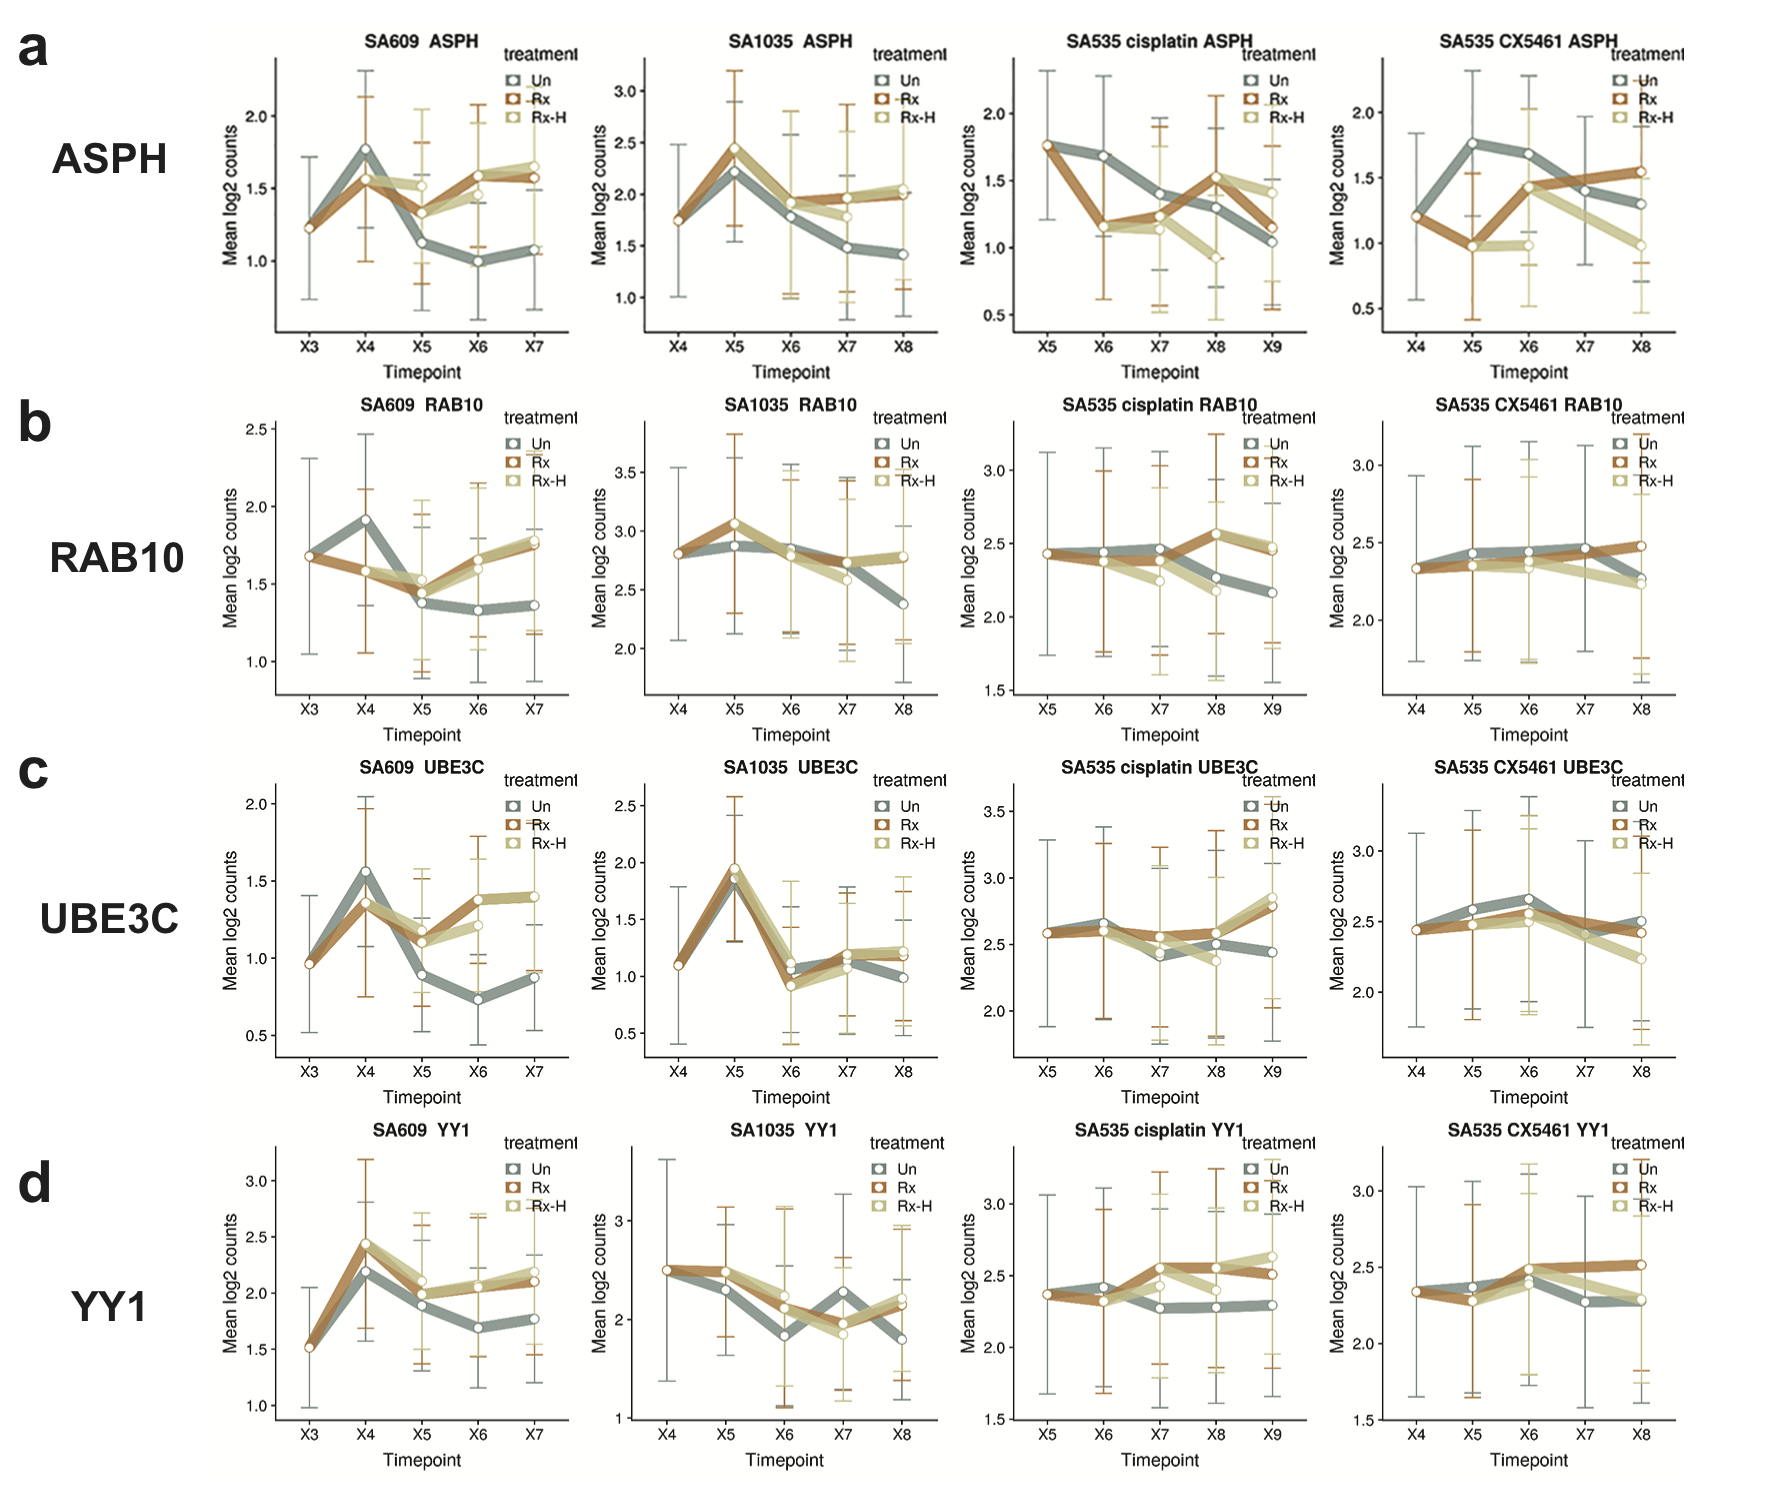
\includegraphics[width=\textwidth]{Figures/chap5/old/commongenesfromvolcanoplots.png}
	
%\caption[Representative trajectories of 4 common genes upregulated in all PDX]
%	{\small
%	\textbf{Representative trajectories of 4 common genes upregulated in all PDXs.}
%	   Horizontal axis shows timepoints passages of tumors. First time point is the baseline untreated value and from second timepoint onwards, depicts increasing cycles of chemotherapy or untreated cycles. Vertical axis represents the SCTransform normalized mean log2 counts of gene expression at that time point. Genes upregulated are selected from \ac{DE} of resistant vs sensitive clones and \textbf{\autoref{tab:UpregulatedgenesinalltreatedPDX}}.
%	   \textbf{(a)} \textit{ASPH} expression trajectories.
%	    \textbf{(b)} \textit{RAB10} expression trajectories.
%	    \textbf{(c)} \textit{UBE3C} expression trajectories.
%	     \textbf{d)} \textit{YY1} expression trajectories.
%	}
%	\label{fig:commongenesfromvolcanoplots}
%\end{figure}
%---------------------------------------------------------------

%\begin{figure}
%\centering
% 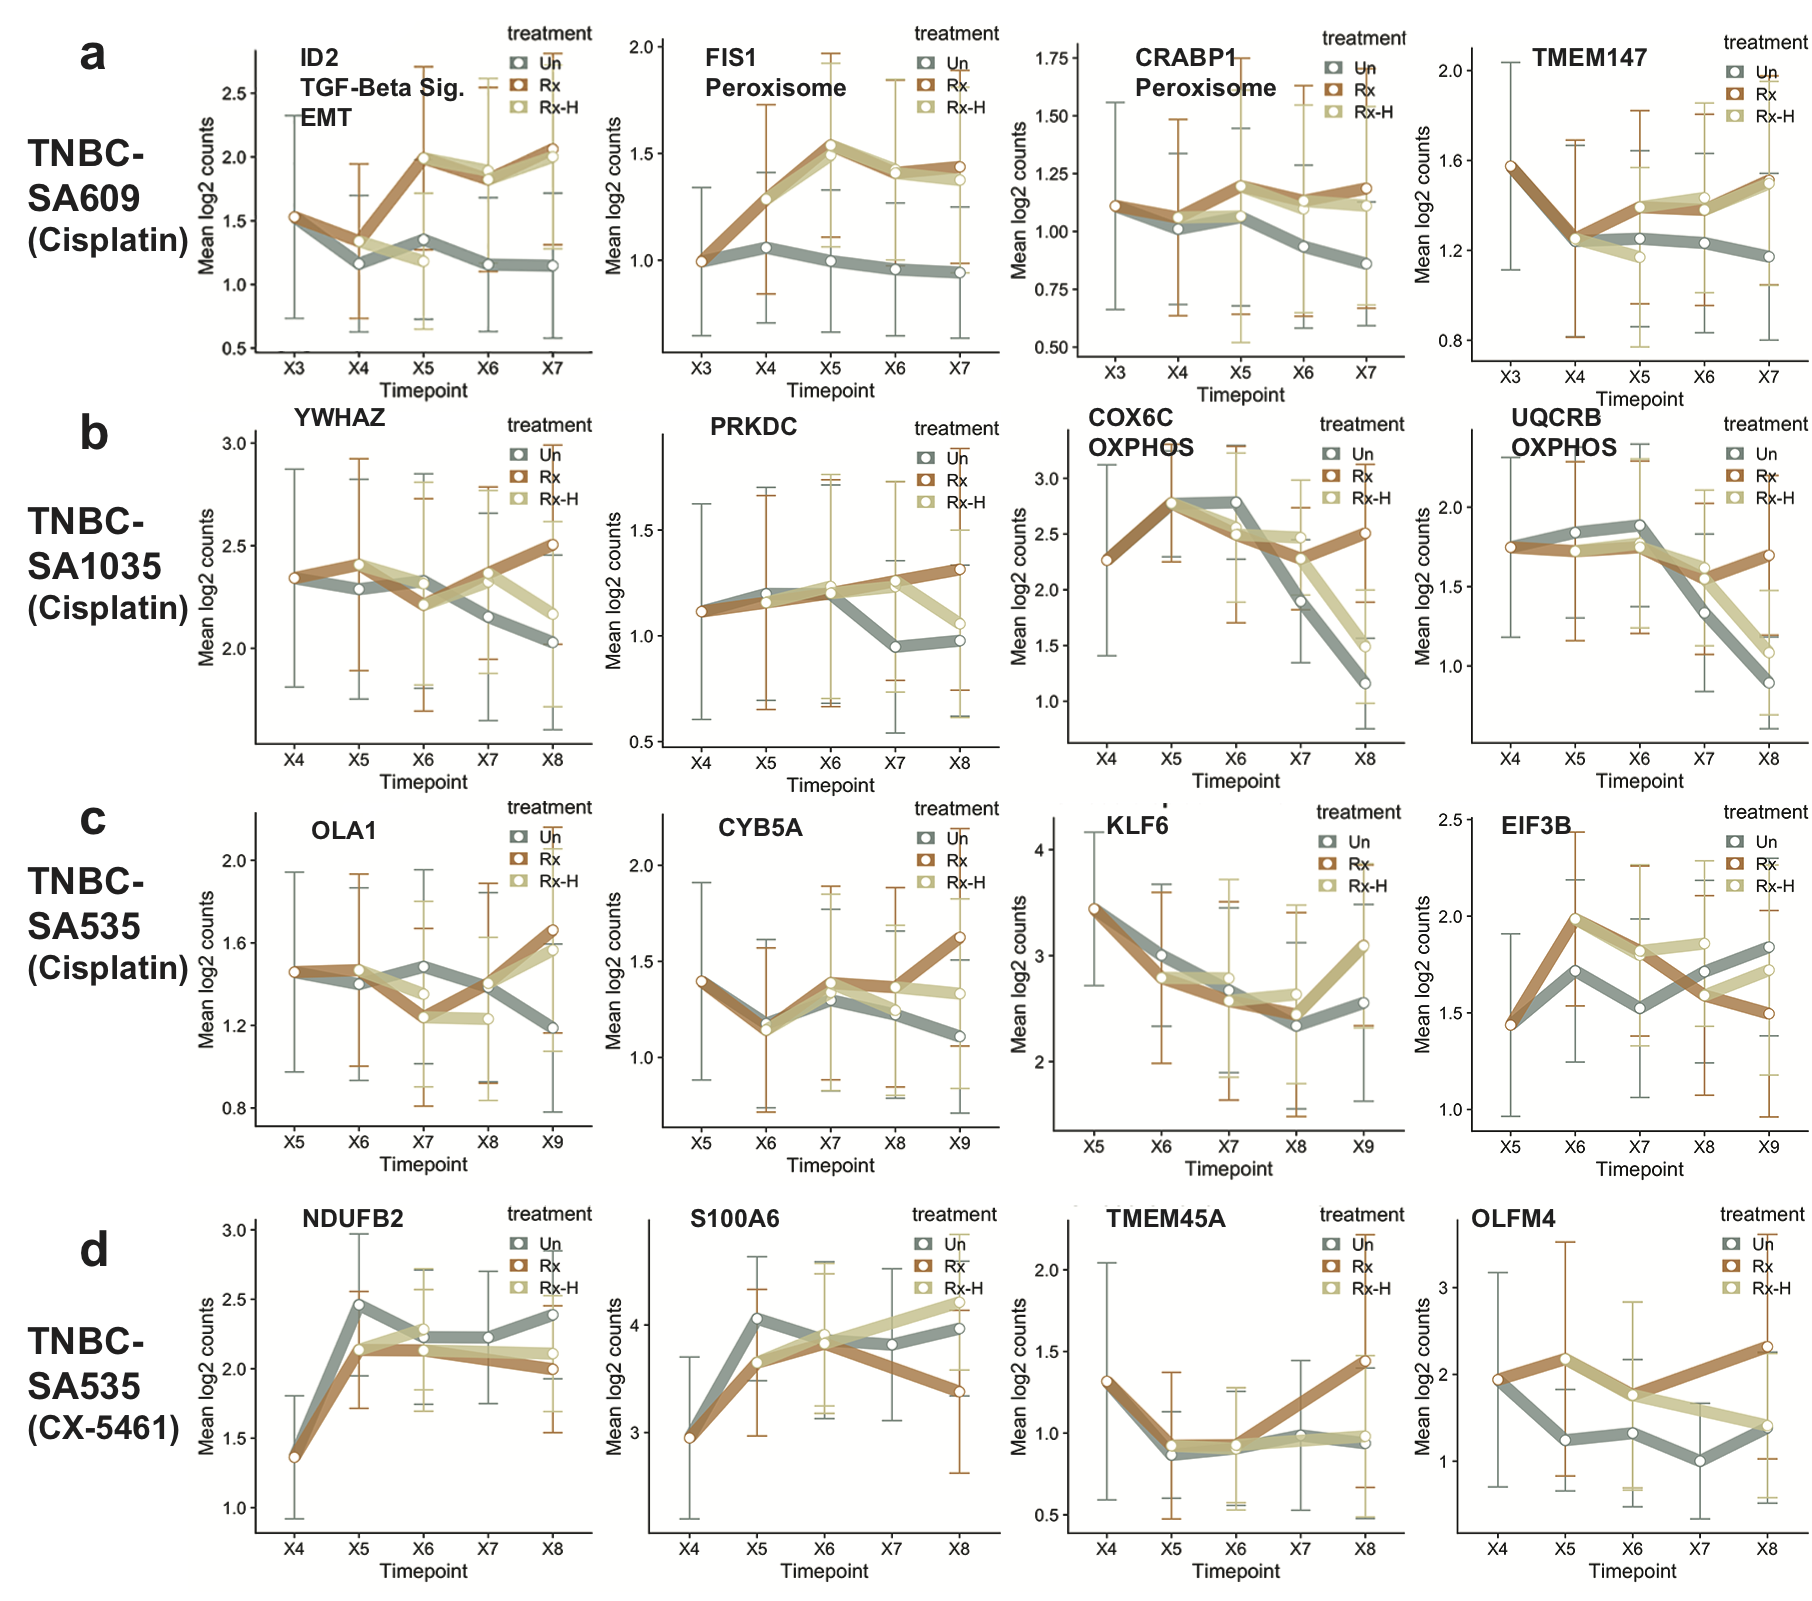
\includegraphics[width=\textwidth]{Figures/chap5/old/incisgenelinetrajectories.png}
%\caption[Four \textit{in cis} gene expression changed over time]
%	{\small
%	 \textbf{Selected four \textit{in cis} regulated gene expression changes over time in all timeseries PDX}.
%	Horizontal axis represents time point passages while vertical axis denotes SCTransform normalized mean log2 counts of single cell expression level. Three line trajectories indicate treated, untreated and drug-holiday samples. }
%	\label{fig:incisgenelinetrajectories}
%\end{figure}
%-----------------------------------------------------------
%\begin{figure}
%\centering
% 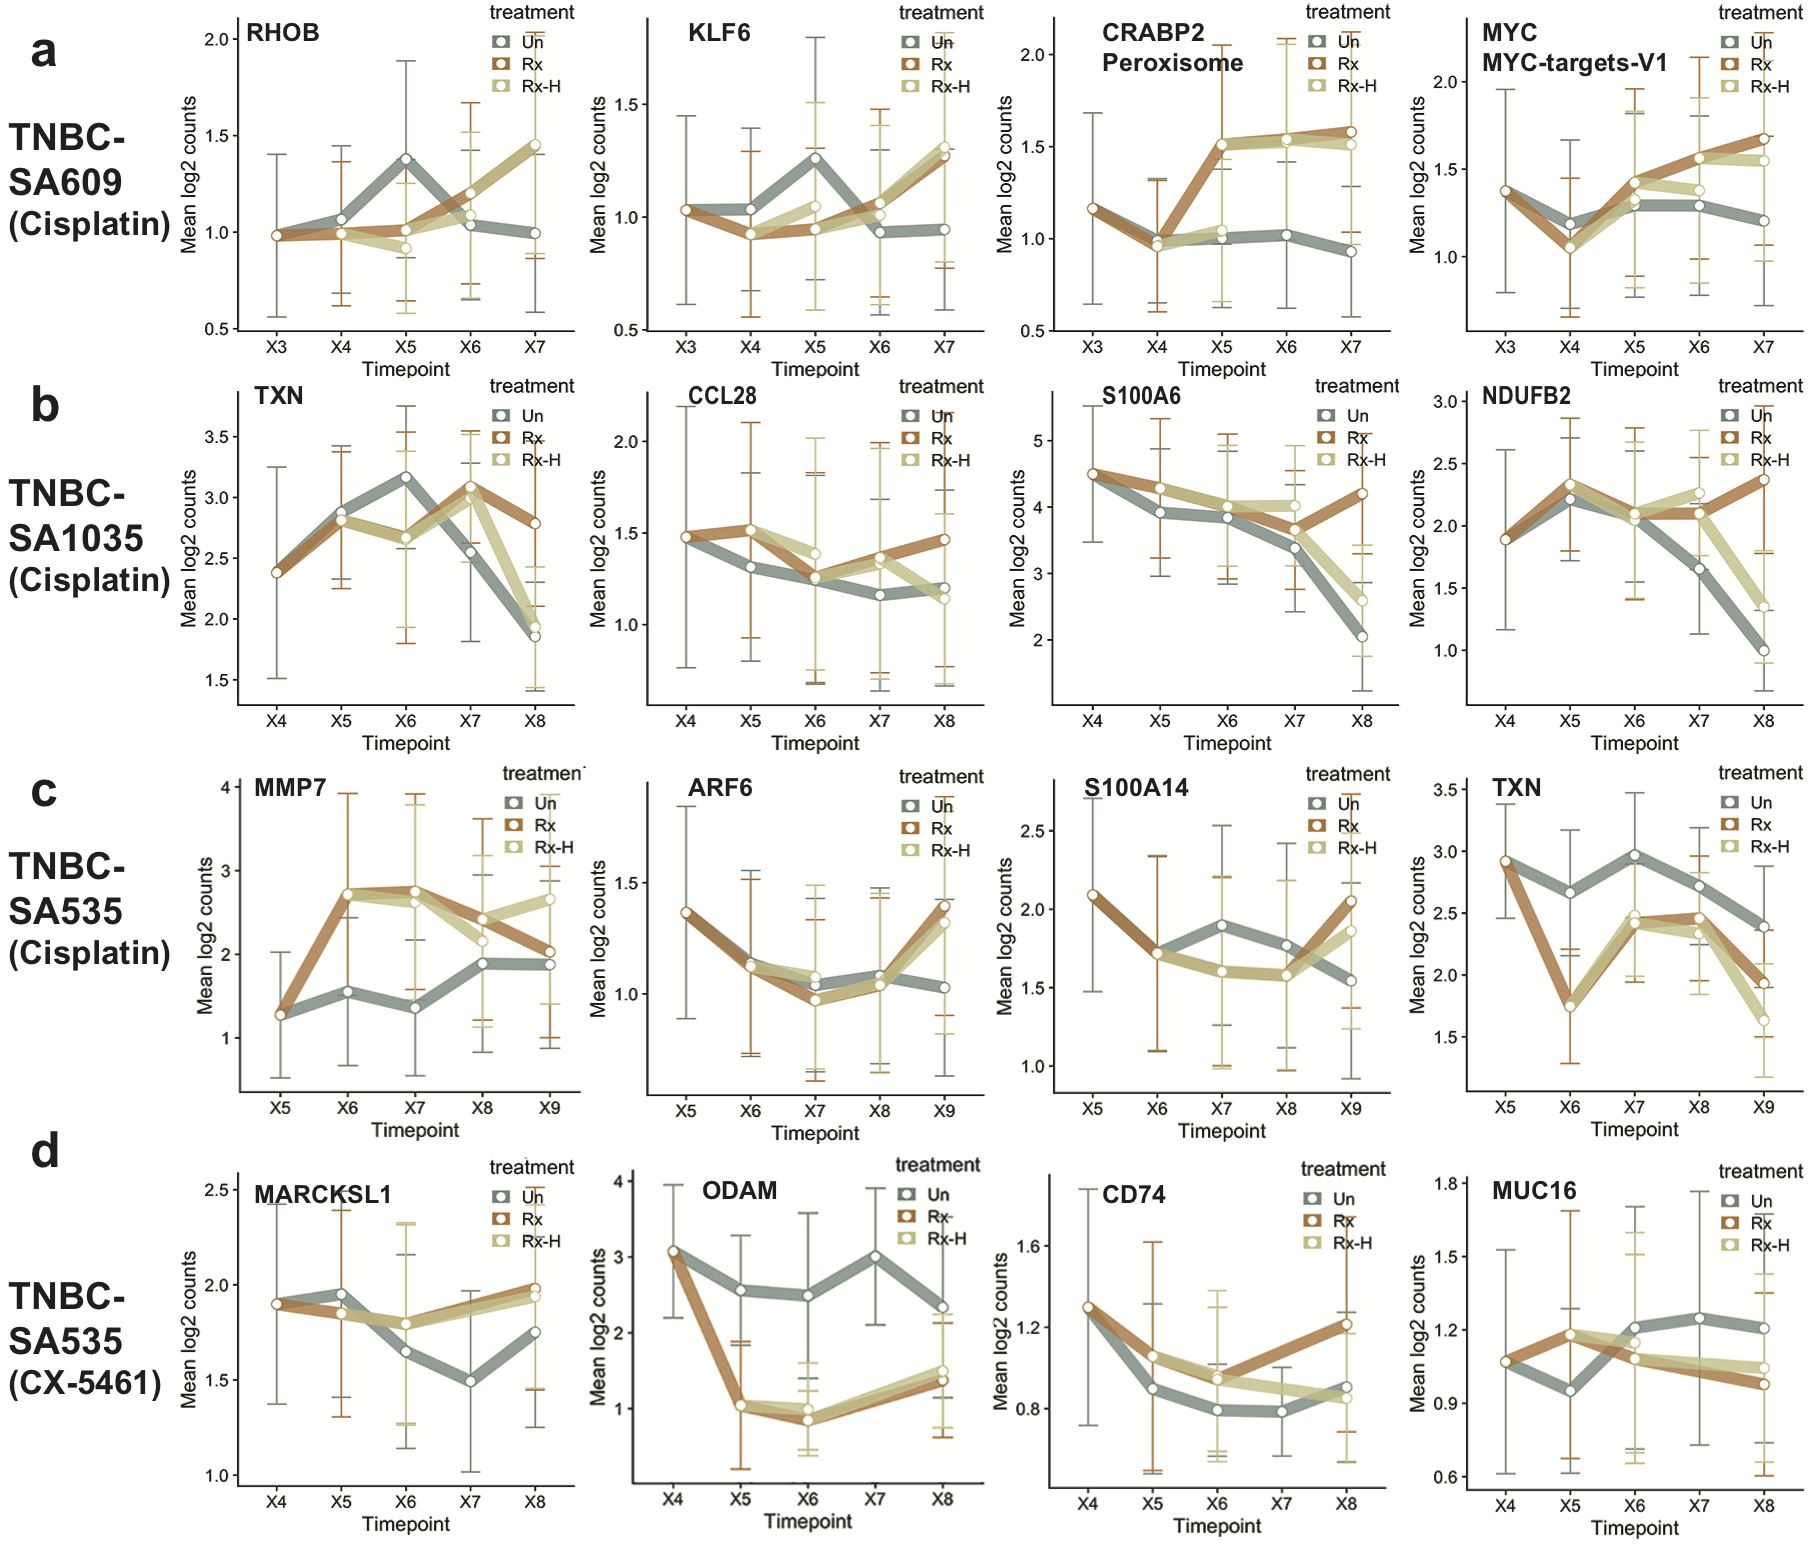
\includegraphics[width=\textwidth]{Figures/chap5/old/Intransgenelinetrajectories.png}
	
%\caption[Four \textit{in trans} gene expression changed over time]
%	{\small
%	 \textbf{Selected four \textit{in trans} regulated gene expression changes over time in all timeseries PDX}.
%	Horizontal axis represents time point passages while vertical axis denotes SCTransform normalized mean log2 count of single cell expression level. Three line trajectories indicates treated, un-treated and drug-holiday samples. }

%	\label{fig:Intransgenelinetrajectories}
%\end{figure} 

%---------------------------------------------------------------
